\documentclass{beamer}
\usepackage{graphicx}
\usepackage{bm}
\usepackage{xcolor}
\usepackage[ruled]{algorithm}
\usepackage{algorithmicx}
\usepackage[noend]{algpseudocode}
\usepackage{amsmath}
\usepackage{amssymb}

\begin{document}
\beamertemplatenavigationsymbolsempty

\title{Temporal Smoothing in 2D Human Pose Estimation for Bouldering}

\author{André Oskar Andersen
\newline \small \texttt{wpr684}}

\institute{Institution of Computer Science, University of Copenhagen}

\date{2023}

\newcommand\unfootnote[1]{%
  \begingroup
  \renewcommand\thefootnote{}\footnote{#1}%
  \addtocounter{footnote}{-1}%
  \endgroup
}

\frame{\titlepage}

\begin{frame}
    \frametitle{Introduction}
    \begin{minipage}{0.5\textwidth}
        \begin{itemize}
            \item<1-> Increased usage of video analysis in sports.
        \end{itemize}
    \end{minipage} \hfill
    \begin{minipage}{0.45\textwidth}
        \begin{figure}
            \center
            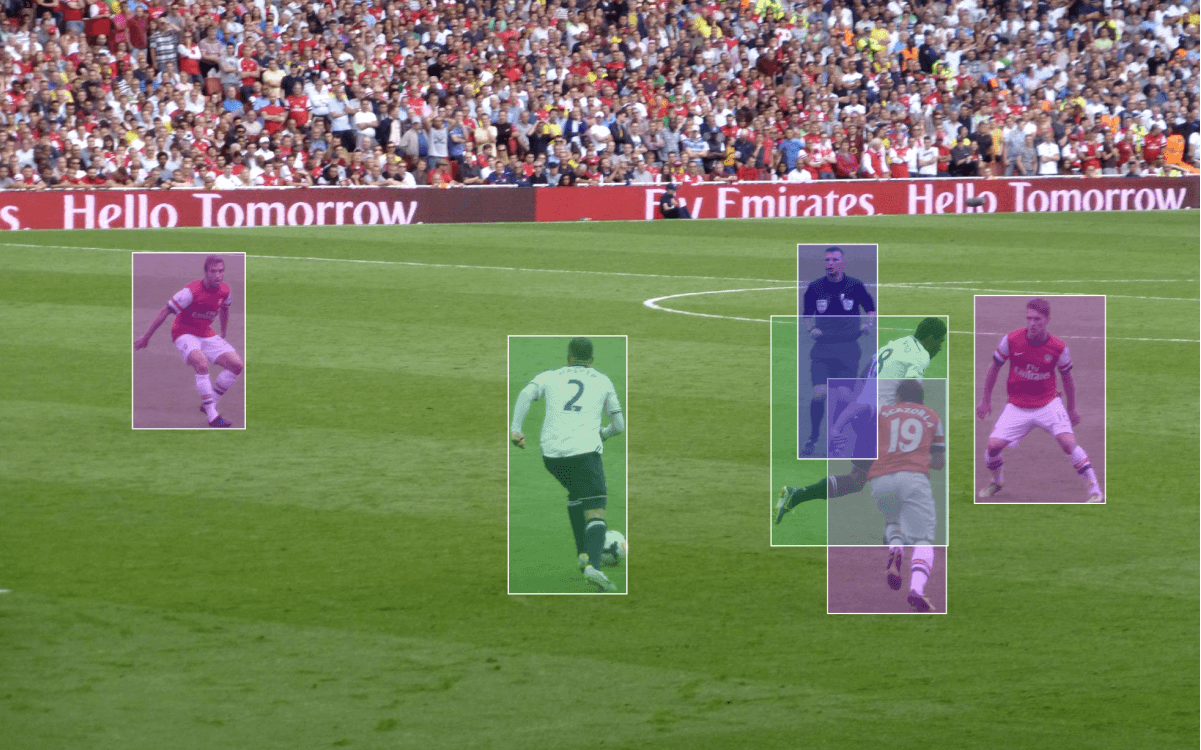
\includegraphics[width = \textwidth]{./entities/soccer_cv.png}
        \end{figure}
    \end{minipage}
    \unfootnote{\tiny \url{https://www.superannotate.com/blog/computer-vision-in-sports}}
\end{frame}

\begin{frame}
    \frametitle{Introduction}
    \begin{minipage}{0.5\textwidth}
        \begin{itemize}
            \item<1-> Increased usage of video analysis in sports.
            \item<1-> Often requires the position of the players.
            \begin{itemize}
                \item Already developed for popular sports.
                \item Missing for the less popular sports.
            \end{itemize}
        \end{itemize}
    \end{minipage} \hfill
    \begin{minipage}{0.45\textwidth}
        \begin{figure}
            \center
            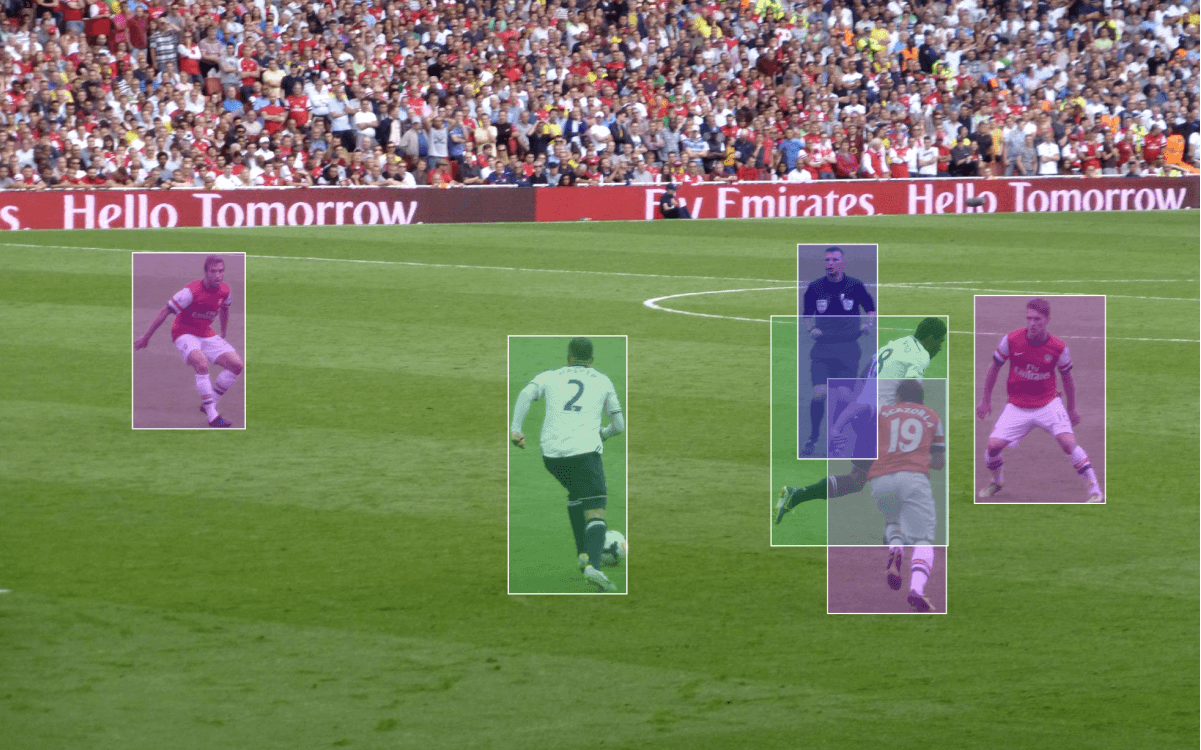
\includegraphics[width = \textwidth]{./entities/soccer_cv.png}
        \end{figure}
    \end{minipage}
    \unfootnote{\tiny \url{https://www.superannotate.com/blog/computer-vision-in-sports}}
\end{frame}

\begin{frame}
    \frametitle{Introduction}
    \begin{minipage}{0.5\textwidth}
        \begin{itemize}
            \item<1-> Increased usage of video analysis in sports.
            \item<1-> Often requires the position of the players.
            \item<1-> Problems with the data
            \begin{itemize}
                \item Methods require large quantities
                \item Unusual poses/movements
            \end{itemize}
        \end{itemize}
    \end{minipage} \hfill
    \begin{minipage}{0.45\textwidth}
        \begin{figure}
            \center
            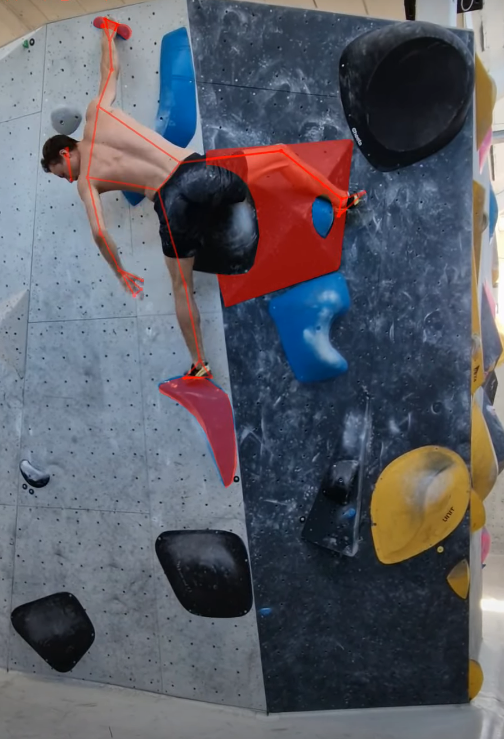
\includegraphics[width = \textwidth]{./entities/ClimbAlong_cv.PNG}
        \end{figure}
    \end{minipage}
    \unfootnote{\tiny \url{https://climbalong.com/lab}}
\end{frame}

\begin{frame}
    \frametitle{Introduction}
    \begin{minipage}{0.5\textwidth}
        \begin{itemize}
            \item<1-> Increased usage of video analysis in sports.
            \item<1-> Often requires the position of the players.
            \item<1-> Problems with the data
            \item<1-> ClimbAlong at NorthTech ApS
            \begin{itemize}
                \item<1-> Frame-idependent pose-detector for bouldering 
                \item<2-> Proposition: Incorporate temporal information
                % TODO: tilføj nogle frames?
            \end{itemize}
        \end{itemize}
    \end{minipage} \hfill
    \begin{minipage}{0.45\textwidth}
        \begin{figure}
            \center
            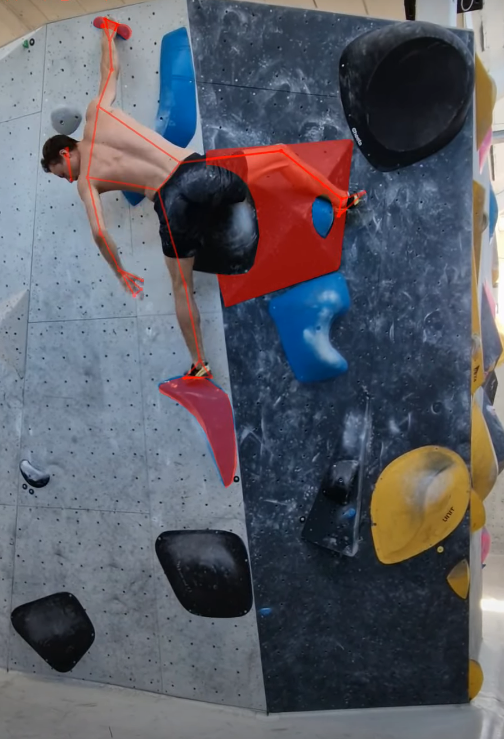
\includegraphics[width = \textwidth]{./entities/ClimbAlong_cv.PNG}
        \end{figure}
    \end{minipage}
    \unfootnote{\tiny \url{https://climbalong.com/lab}}
\end{frame}

\begin{frame}
    \frametitle{Introduction}
    \begin{itemize}
        \item<1-> Aim: extending the ClimbAlong pose-detector to use temporal information.
    \end{itemize}
\end{frame}

\begin{frame}
    \frametitle{The Data}
    \begin{minipage}{0.5\textwidth}
        ClimbAlong
        \begin{itemize}
            \item Fully annoated videos of climbers
            \item<2-> Problem: Very small dataset
            \item<3-> Solution: pretrain on related datasets and finetune on ClimbAlong
            \begin{itemize}
                \item BRACE
                \item Penn Action
            \end{itemize}
            % TODO: tilføj visualizations
        \end{itemize}
    \end{minipage} \hfill
    \begin{minipage}{0.45\textwidth}
        \begin{figure}
            \center
            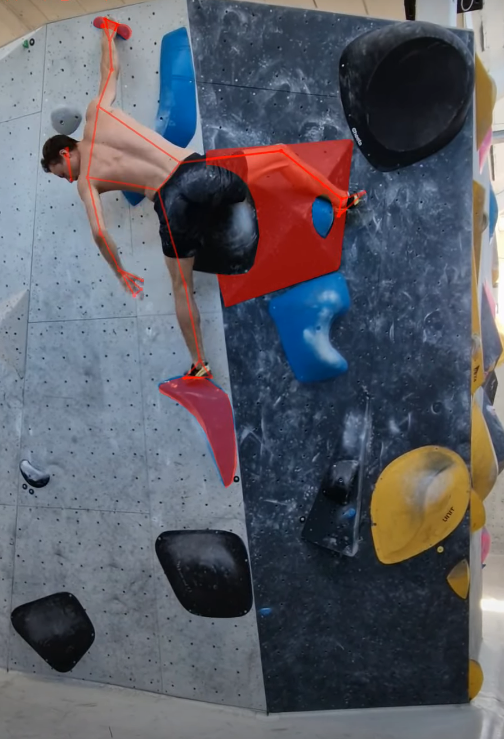
\includegraphics[width = \textwidth]{./entities/ClimbAlong_cv.PNG}
        \end{figure}
    \end{minipage}
    \unfootnote{\tiny \url{https://climbalong.com/lab}}
\end{frame}

\begin{frame}
    \frametitle{The Data}
    \begin{minipage}{0.5\textwidth}
        ClimbAlong
        \begin{itemize}
            \item Fully annoated videos of climbers
            \item Problem: Very small dataset
            \item Solution: pretrain on related datasets and finetune on ClimbAlong
            \begin{itemize}
                \item BRACE
                \item Penn Action
            \end{itemize}
            % TODO: tilføj visualizations
        \end{itemize}
    \end{minipage} \hfill
    \begin{minipage}{0.45\textwidth}
        \begin{figure}
            \center
            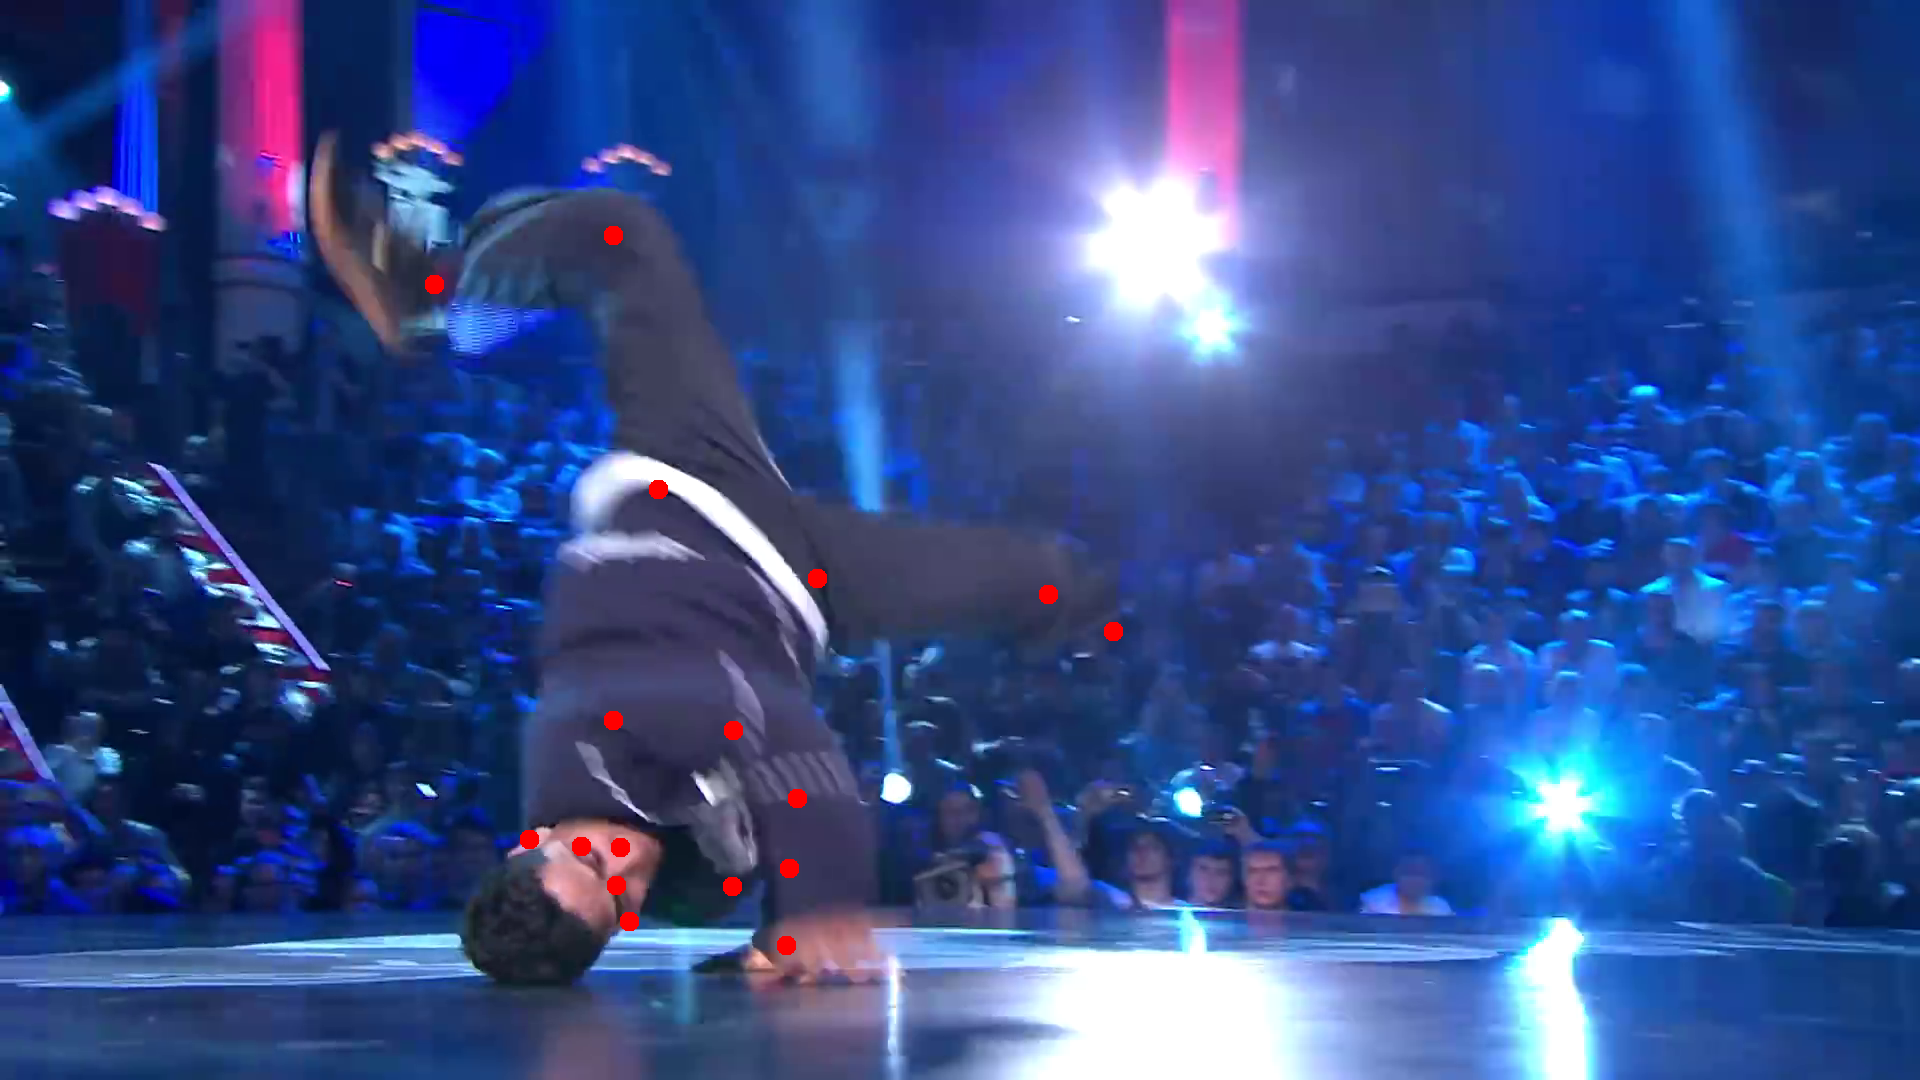
\includegraphics[width = \textwidth]{../report/entities/BRACE_1152.png}
            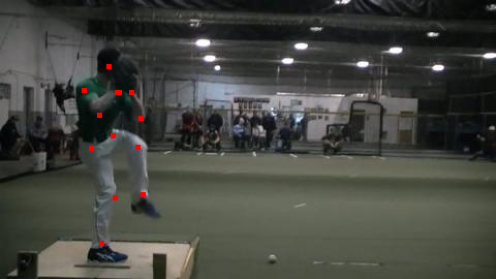
\includegraphics[width = \textwidth]{../report/entities/PA_64.png}
        \end{figure}
    \end{minipage}
\end{frame}

\begin{frame}
    \frametitle{The Models}
    Generally, three approaches
    \begin{enumerate}
        \item Convolutional layer
        \item Recurrent neural network
        \item Transformer
    \end{enumerate}
\end{frame}

\begin{frame}
    \frametitle{The Models}
    3DConv
    \begin{itemize}
        \item<1-> 3-dimensional conv. layer + ReLU
    \end{itemize}
    \begin{figure}
        \centering
        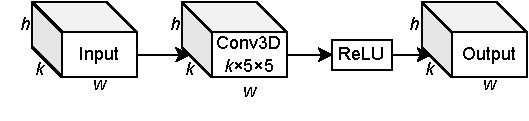
\includegraphics[width = 0.8\textwidth]{../report/entities/baseline.pdf}
    \end{figure}
    \unfootnote{\tiny \url{https://arxiv.org/pdf/2203.08713.pdf}}
\end{frame}

\begin{frame}
    \frametitle{The Models}
    bi-ConvLSTM Model S
    \begin{itemize}
        \item<1-> Adaptation of Unipose-LSTM by Artacho and Savakis
        \item<1-> Bidirectional convolutional LSTM + conv. layers and ReLU
        \item<1-> Processing directions summed together
    \end{itemize}
    \begin{figure}
        \centering
        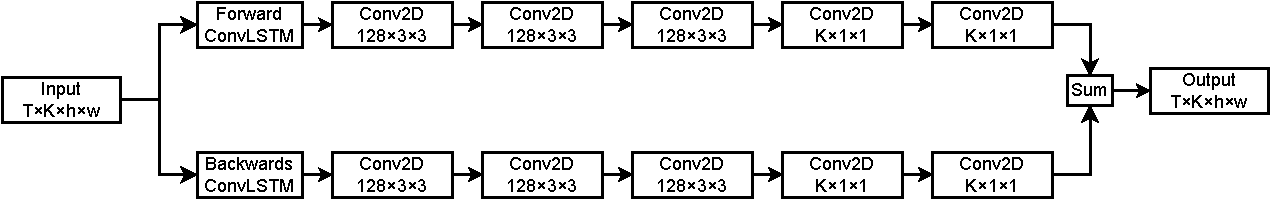
\includegraphics[width = \textwidth]{../report/entities/bi_conv_lstm.pdf}
    \end{figure}
\end{frame}

\begin{frame}
    \frametitle{The Models}
    bi-ConvLSTM Model C
    \begin{itemize}
        \item<1-> Problem: Prioritization of processing direction
        \item<1-> Solution: Using convolution
    \end{itemize}
    \begin{figure}
        \centering
        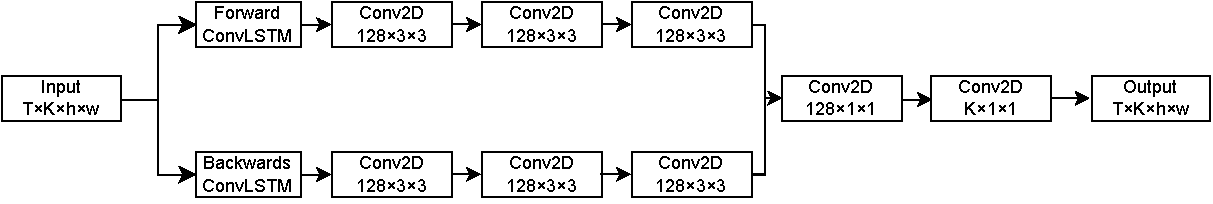
\includegraphics[width = \textwidth]{../report/entities/unipose2.pdf}
    \end{figure}
\end{frame}

\begin{frame}
    \frametitle{The Models}
    DeciWatch by Zeng \textit{Et al}.
    \begin{itemize}
        \item<1-> Transformer-based
        \item<1-> Only considers every $n$th frame
        \item<1-> Encoder: DenoiseNet
        \item<1-> Decoder: RecoverNet
    \end{itemize}
    \begin{figure}
        \centering
        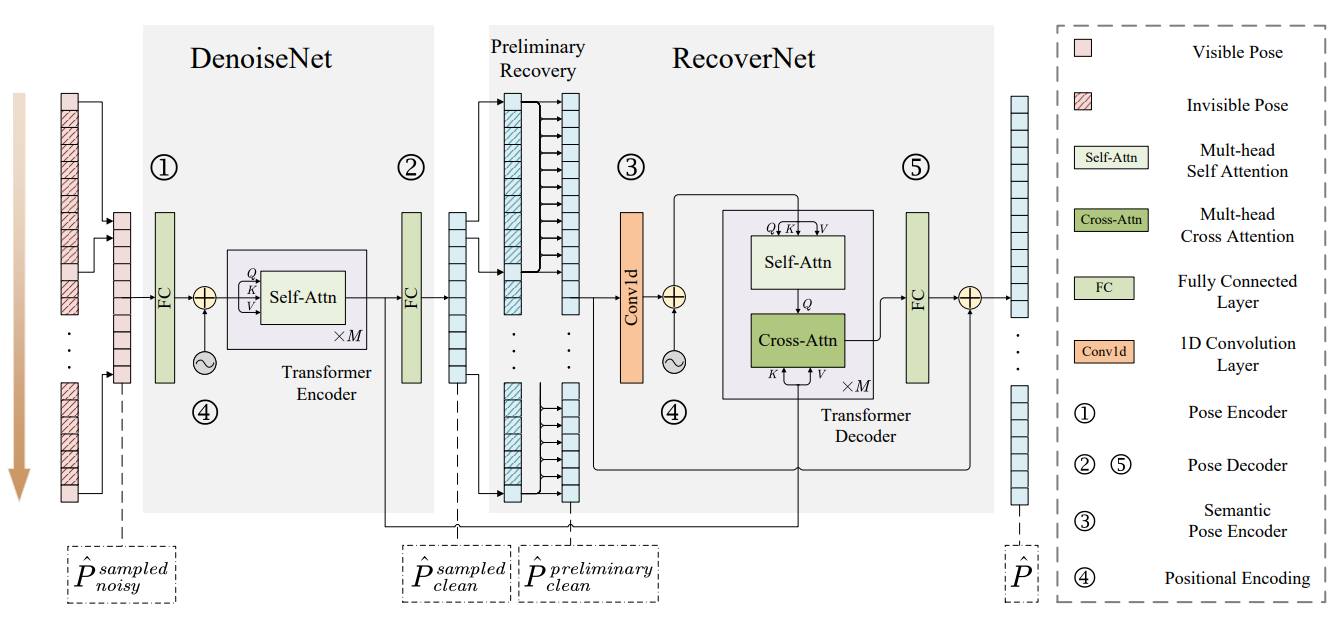
\includegraphics[width = \textwidth]{../report/entities/deciwatch.PNG}
    \end{figure}
\end{frame}

\begin{frame}
    \frametitle{Pretraining}
    Procedure
    \begin{itemize}
        \item<1-> Not training pose-detector
        \begin{enumerate}
            \item Different input images
        \end{enumerate}
        \item<2-> Simulating pose-detector output by adding noise
        \begin{enumerate}
            \item Gaussian filter standard deviation
            \item Shifting keypoints
        \end{enumerate}
    \end{itemize}
    \only<2>{
        \begin{figure}
            \centering
            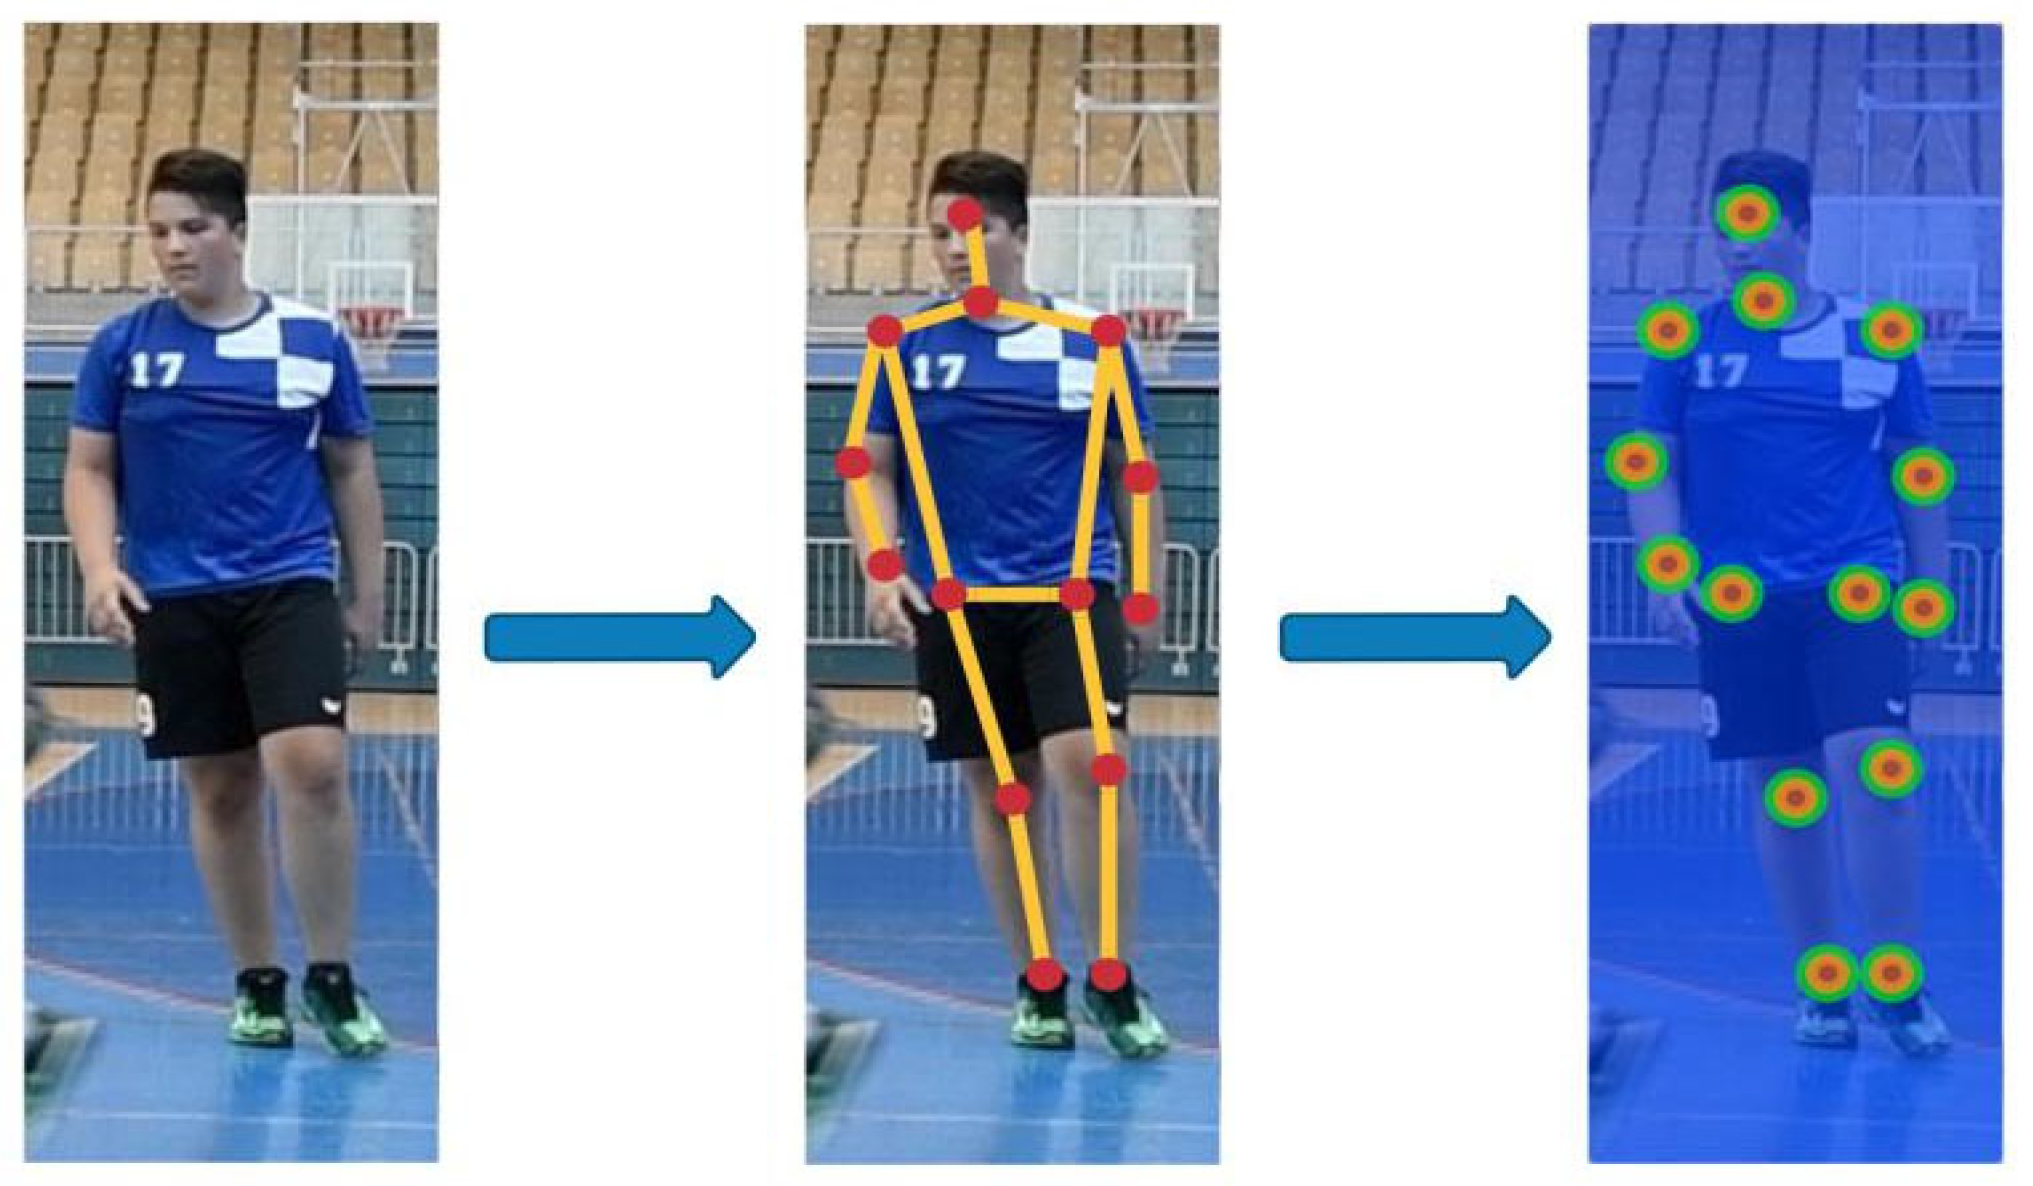
\includegraphics[width = 0.7 \textwidth]{./entities/heatmaps.png}
        \end{figure}
        \unfootnote{\tiny \url{https://www.mdpi.com/2313-433X/8/11/308}}
    }
\end{frame}

\begin{frame}
    \frametitle{Pretraining}
    Finding optimal setting of models
    \begin{itemize}
        \item<1-> Three experiments
        \begin{enumerate}
            \item<1-> Sample Gaussian filter standard deviation from $\{1, 1.5, 2, 2.5, 3\}$.
            \item<2-> Fixed standard deviation
            \item<3-> Decreased frame rate
        \end{enumerate}
        \item<4-> Shifting by sampling from $\mathcal{N}(\mu = 0, \sigma = 3k)$ for $k \in \{1, 2\}$
    \end{itemize}
\end{frame}

\begin{frame}
    \frametitle{Finetuning}
    \begin{itemize}
        \item<1-> Using all of the developed models with pose-detector
        \item<1-> Freezing pose-detector
        \begin{enumerate}
            \item Quicker fitting
            \item Greater understanding of results  
        \end{enumerate}
    \end{itemize}
\end{frame}

\begin{frame}
    \frametitle{Finetuning}
    \begin{itemize}
        \item<1-> Test results
    \end{itemize}
\end{frame}

\begin{frame}
    \frametitle{Discussion}
    Results:
    \begin{itemize}
        \item<1-> Translation vs translation + scaling
        \item<2-> Halfing frame rate
        \item<3-> Easiest vs most difficult joints
        \item<4-> Experiment 1 vs experiment 2
        \item<5-> Effects of pretraining
        \item<6-> Worst performing keypoints
    \end{itemize}
\end{frame}

\begin{frame}
    \frametitle{Discussion}
    All models performed better during finetuning than pretraining
    \begin{enumerate}
        \item<1-> More data
        \item<2-> Semantically different videos in pretraining
        \item<3-> Noise in BRACE annotations
        \item<4-> Frame rate in Penn Action
        \item<5-> Performace of identity function
    \end{enumerate}
\end{frame}

\begin{frame}
    \frametitle{Discussion}
    Which model is the best?
    \begin{itemize}
        \item<1-> Greatest testing accuracy: DeciWatch 1.1/1.2
        \item<2-> Greatest rough estimation: bi-ConvLSTM Model C 1.1
        \item<3-> Speed and memory: 3DConv
    \end{itemize}
\end{frame}

\begin{frame}
    \frametitle{Discussion}
    General reflections
    \begin{itemize}
        \item<1-> Pretraining
        \begin{itemize}
            \item<1-> Should have estimated parameters of data
            \item<2-> Overlapping video sequences
        \end{itemize}
        \item<3-> Finetuning
        \begin{itemize}
            \item<3-> Groundtruth outside of bbox 
        \end{itemize}
    \end{itemize}
\end{frame}

\begin{frame}
    \frametitle{Discussion}
    Future work
    \begin{enumerate}
        \item<1-> DeciWatch with all frames
        \item<2-> DeciWatch with vision transformer
        \item<3-> Avoid overfitting
        \item<4-> Multiple retraining
    \end{enumerate}
\end{frame}

\begin{frame}
    \frametitle{Conclusion}
    Succesfully developed and tested the incorporation of temporal smoothing for pose estimation
\end{frame}

\begin{frame}
    \frametitle{Extras: Mistakes Were Made!}
    Misimplemented evaluation-function
\end{frame}

\end{document}